% !TEX root = ./main.tex

% =========================================================
% 西南财经大学本科生毕业论文（设计）宏包配置与全局格式
% 依据：《西南财经大学本科生毕业论文（设计）撰写与印制规范》
% =========================================================

% 使用发行版提供的文档类，拒绝旧接口版本。
\IfClassAtLeastTF{sjtuthesis}{2026/02/26}{}{%
  \PackageError{swufe}{SJTUTeX 2.3.1 or newer is required}%
    {Update the sjtutex package in your TeX distribution.\MessageBreak
     On Overleaf, select TeX Live 2026 or newer.}%
}

\ExplSyntaxOn

% ---------------------------------------------------------
% 1. 本科论文信息与开关（单套字段，不区分语言）
% ---------------------------------------------------------
\tl_new:N \l__swufe_info_grade_tl
\tl_new:N \l__swufe_info_final_date_tl
\tl_new:N \l__swufe_info_display_title_tl
\tl_new:N \l__swufe_info_title_second_tl
\bool_new:N \g__swufe_citation_superscript_bool
\bool_new:N \g__swufe_bibliography_bib_bool
\tl_new:N \l__swufe_bibliography_bib_file_tl
\tl_new:N \l__swufe_bibliography_tex_file_tl

\keys_define:nn { sjtu }
  {
    review              .bool_gset:N = \g__sjtu_review_bool ,
    citation-superscript .bool_gset:N = \g__swufe_citation_superscript_bool ,
    bibliography .meta:nn = { sjtu / bibliography } {#1} ,
  }
\keys_define:nn { sjtu / bibliography }
  {
    source .choice: ,
    source / bib .code:n = { \bool_gset_true:N \g__swufe_bibliography_bib_bool } ,
    source / tex .code:n = { \bool_gset_false:N \g__swufe_bibliography_bib_bool } ,
    bib-file .tl_set:N = \l__swufe_bibliography_bib_file_tl ,
    tex-file .tl_set:N = \l__swufe_bibliography_tex_file_tl ,
  }
\keys_define:nn { sjtu / info }
  {
    % 修改完整标题时清空封面分行；后续可用两个可选字段重新指定。
    title .code:n =
      {
        \tl_set:cn { l__sjtu_info_title_zh_tl } {#1}
        \tl_clear:N \l__swufe_info_display_title_tl
        \tl_clear:N \l__swufe_info_title_second_tl
      } ,
    % 新版文档类要求显式语言；对外仍保留本科模板的单套字段。
    subject    .meta:nn = { sjtu / info / zh } { subject = {#1} } ,
    keywords   .meta:nn = { sjtu / info / zh } { keywords = {#1} } ,
    author     .meta:nn = { sjtu / info / zh } { author = {#1} } ,
    id         .meta:nn = { sjtu / info / zh } { id = {#1} } ,
    department .meta:nn = { sjtu / info / zh } { department = {#1} } ,
    major      .meta:nn = { sjtu / info / zh } { major = {#1} } ,
    supervisor .meta:nn = { sjtu / info / zh } { supervisor = {#1} } ,
    grade         .tl_set:N = \l__swufe_info_grade_tl ,
    final-date    .tl_set:N = \l__swufe_info_final_date_tl ,
    display-title .tl_set:N = \l__swufe_info_display_title_tl ,
    title-second  .tl_set:N = \l__swufe_info_title_second_tl ,
  }

\cs_set_eq:NN \swufesetup \sjtusetup

% 本科模板的单套字段映射到中文主语言信息；内部存储细节不暴露到配置中。
\newcommand{\swufetitle}{\tl_use:c { l__sjtu_info_title_zh_tl }}
\newcommand{\swufeauthor}{\tl_use:c { l__sjtu_info_author_zh_tl }}
\newcommand{\swufesupervisor}{\tl_use:c { l__sjtu_info_supervisor_zh_tl }}
\newcommand{\swufedepartment}{\tl_use:c { l__sjtu_info_department_zh_tl }}
\newcommand{\swufemajor}{\tl_use:c { l__sjtu_info_major_zh_tl }}
\newcommand{\swufeid}{\tl_use:c { l__sjtu_info_id_zh_tl }}
\newcommand{\swufegrade}{\tl_use:N \l__swufe_info_grade_tl}
\newcommand{\swufetitlesecond}{\tl_use:N \l__swufe_info_title_second_tl}
\newcommand{\swufedisplaytitle}{%
  \tl_if_empty:NTF \l__swufe_info_display_title_tl
    { \swufetitle }
    { \tl_use:N \l__swufe_info_display_title_tl }%
}
\newcommand{\swufefinaldate}{%
  \tl_if_empty:NTF \l__swufe_info_final_date_tl
    { \tl_use:c { l__sjtu_info_date_zh_tl } }
    { \tl_use:N \l__swufe_info_final_date_tl }%
}

\newif\ifswufereview
\cs_new_protected:Npn \__swufe_sync_review_status:
  {
    \bool_if:NTF \g__sjtu_review_bool
      { \swufereviewtrue }
      { \swufereviewfalse }
  }
\ctex_at_end_preamble:n
  {
    \__swufe_sync_review_status:
    % 盲审开关在 JSON 加载后才确定，同步 PDF 作者元数据。
    \bool_if:NTF \g__sjtu_review_bool
      { \cs_set:cpn { @author } { } }
      { \cs_set:cpn { @author } { \swufeauthor } }
  }
\ExplSyntaxOff

% ---------------------------------------------------------
% 2. 默认设置（config.json 中已提供的字段覆盖对应默认值）
% ---------------------------------------------------------
\swufesetup{
  review = false,
  citation-superscript = false,
  bibliography = {
    source = bib,
    bib-file = refs.bib,
    tex-file = contents/参考文献.tex,
  },
  info = {
    title         = {西南财经大学本科毕业论文（设计）\LaTeX{} 模板示例文档},
    display-title = {西南财经大学本科毕业论文（设计）},
    title-second  = {\LaTeX{} 模板示例文档},
    subject       = {西南财经大学本科毕业论文（设计）},
    keywords      = {西南财经大学, 本科毕业论文, LaTeX 模板, 排版规范},
    author        = {张\quad{}三},
    id            = {42100001},
    department    = {计算机与人工智能学院},
    major         = {计算机科学与技术},
    grade         = {2022级},
    supervisor    = {李四\quad{}教授},
    final-date    = {2026年5月},
  }
}

% ---------------------------------------------------------
% 3. JSON 配置加载（仅接受 config.json 中的统一字段）
% ---------------------------------------------------------
\IfFileExists{config.json}{%
  \RequirePackage{jsonparse}
  \JSONParseFromFile{\swufeJsonData}{config.json}
}{ }
\ExplSyntaxOn
\file_if_exist:nT { config.json }
  {
    % 同一入口读取字符串与布尔值；空字符串可用于清空可选字段。
    \cs_new_protected:Npn \__swufe_load_json_field:nnn #1#2#3
      {
        \prop_if_in:NnT \swufeJsonData {#3}
          {
            % 重新分词 LaTeX 命令时保留标题、姓名中的普通空格。
            \group_begin:
              \char_set_catcode_space:n { 32 }
              \JSONParseSetRescanValue \l_tmpa_tl \swufeJsonData {#3}
              \exp_args:NNNV \group_end: \tl_set:Nn \l_tmpa_tl \l_tmpa_tl
            \keys_set:nx {#1} { #2 = { \exp_not:V \l_tmpa_tl } }
          }
      }
    \clist_map_inline:nn
      {
        { review }              { review } ,
        { citation-superscript } { citation_superscript }
      }
      { \__swufe_load_json_field:nnn { sjtu } #1 }
    \clist_map_inline:nn
      {
        { source }   { bibliography.source } ,
        { bib-file } { bibliography.bib_file } ,
        { tex-file } { bibliography.tex_file }
      }
      { \__swufe_load_json_field:nnn { sjtu / bibliography } #1 }
    \clist_map_inline:nn
      {
        { title }         { info.title } ,
        { display-title } { info.display_title } ,
        { title-second }  { info.title_second } ,
        { keywords }      { info.keywords } ,
        { author }        { info.author } ,
        { id }            { info.student_id } ,
        { department }    { info.department } ,
        { major }         { info.major } ,
        { grade }         { info.grade } ,
        { supervisor }    { info.supervisor } ,
        { final-date }    { info.final_date }
      }
      { \__swufe_load_json_field:nnn { sjtu / info } #1 }
  }
\__swufe_sync_review_status:
\ExplSyntaxOff

% ---------------------------------------------------------
% 4. 页面尺寸与全文页边距
% 规范要求：A4 纸，全文页边距：上3厘米，下3厘米，左3厘米，右3厘米。
% ---------------------------------------------------------
\usepackage{geometry}
\geometry{
  a4paper,
  bindingoffset = 0pt, % 清除文档类默认的 0.5cm 装订偏移，保证左右均为 3cm
  top           = 3.0cm,
  bottom        = 3.0cm,
  left          = 3.0cm,
  right         = 3.0cm,
  headheight    = 15pt,
  headsep       = 18pt,
  footskip      = 1.0cm
}

% ---------------------------------------------------------
% 5. 字体配置
% 规范要求：华文中宋（一级标题、中英文摘要标题、目录标题等）、宋体（正文）、黑体（二级、三级标题及图表题）
% ---------------------------------------------------------
\usepackage{fontspec}

% 西文字体：完整的项目字体组 -> 系统 Times New Roman -> TeX Gyre TermesX。
% 四种字形作为一组检查，缺少任意文件时整组回退，避免粗体或斜体加载失败。
\newif\ifswufetimesfiles
\swufetimesfilestrue
\IfFileExists{font/Times New Roman.ttf}{}{\swufetimesfilesfalse}
\IfFileExists{font/Times New Roman Bold.ttf}{}{\swufetimesfilesfalse}
\IfFileExists{font/Times New Roman Italic.ttf}{}{\swufetimesfilesfalse}
\IfFileExists{font/Times New Roman Bold Italic.ttf}{}{\swufetimesfilesfalse}
\ifswufetimesfiles
  \setmainfont[
    Path = font/,
    UprightFont    = {Times New Roman.ttf},
    BoldFont       = {Times New Roman Bold.ttf},
    ItalicFont     = {Times New Roman Italic.ttf},
    BoldItalicFont = {Times New Roman Bold Italic.ttf}
  ]{}
\else
  \IfFontExistsTF{Times New Roman}{
    \setmainfont{Times New Roman}
  }{
    \setmainfont[
      Extension = .otf,
      UprightFont = *-Regular,
      BoldFont = *-Bold,
      ItalicFont = *-Italic,
      BoldItalicFont = *-BoldItalic
    ]{TeXGyreTermesX}
    \PackageWarningNoLine{swufe}{Times New Roman unavailable; using TeX Gyre TermesX}
  }
\fi

% 一级标题字体：项目华文中宋 -> 系统华文中宋 -> Fandol 宋体。
% 华文中宋没有独立粗体，使用合成加粗；Fandol 使用其自带粗体。
\IfFileExists{font/STZHONGS.TTF}{
  \setCJKfamilyfont{zhongsong}[Path=font/,AutoFakeBold=2.5]{STZHONGS.TTF}
}{
  \IfFontExistsTF{STZhongsong}{
    \setCJKfamilyfont{zhongsong}[AutoFakeBold=2.5]{STZhongsong}
  }{
    \setCJKfamilyfont{zhongsong}[BoldFont=FandolSong-Bold.otf]{FandolSong-Regular.otf}
    \PackageWarningNoLine{swufe}{STZhongsong unavailable; using FandolSong}
  }
}
\newcommand{\zhongsong}{\CJKfamily{zhongsong}}

% 封面字体：项目华文仿宋 -> 系统华文仿宋 -> Fandol 仿宋。
\IfFileExists{font/STFANGSO.TTF}{
  \setCJKfamilyfont{hwfangsong}[Path=font/,AutoFakeBold=2]{STFANGSO.TTF}
}{
  \IfFontExistsTF{STFangsong}{
    \setCJKfamilyfont{hwfangsong}[AutoFakeBold=2]{STFangsong}
  }{
    \setCJKfamilyfont{hwfangsong}[AutoFakeBold=2]{FandolFang-Regular.otf}
    \PackageWarningNoLine{swufe}{STFangsong unavailable; using FandolFang}
  }
}
\newcommand{\hwfangsong}{\CJKfamily{hwfangsong}}

% 华文行楷 / 楷书回退定义（用于封底校训竖排）
\providecommand{\hwxingkai}{\kaishu}
\IfFileExists{font/STXINGKA.TTF}{
  \setCJKfamilyfont{hwxingkai}[Path=font/]{STXINGKA.TTF}
  \renewcommand{\hwxingkai}{\CJKfamily{hwxingkai}}
}{
  \IfFontExistsTF{STXingkai}{
    \setCJKfamilyfont{hwxingkai}{STXingkai}
    \renewcommand{\hwxingkai}{\CJKfamily{hwxingkai}}
  }{}
}

% ---------------------------------------------------------
% 6. 行距与段落格式
% 规范要求：正文小四号宋体，行距1.5倍，段前0，段后0，首行缩进2字符，两端对齐
% ---------------------------------------------------------
\usepackage{setspace}
% 使用 CTeX 的单倍基线（字号的 1.2 倍），再乘 1.5；
% main.tex 禁用文档类默认的固定 20bp 基线，避免重复放大。
\setstretch{1.5}
% 标题段前、段后“行”统一以小四号正文的实际基线间距计量。
\newlength{\swufebodyline}
\begingroup
  \normalsize
  \global\swufebodyline=\baselineskip
\endgroup
\setlength{\parindent}{2\ccwd}
\setlength{\parskip}{0pt}

% ---------------------------------------------------------
% 7. 各级标题样式设置
% 规范要求：
% 一级标题：二号华文中宋加粗，居中，段前3行，段后2行，1.5倍行距，编号如“1. ……”或“1 ……”
% 二级标题：小三号黑体，首行无缩进，段前1行，段后1行，1.5倍行距，编号如“1.1 ……”
% 三级标题：小四号黑体，首行无缩进，段前1行，段后1行，1.5倍行距，编号如“1.1.1 ……”
% ---------------------------------------------------------
\ctexset{
  chapter = {
    name        = {},
    number      = \arabic{chapter},
    aftername   = {\ },
    format      = \normalfont\centering\zhongsong\bfseries\setstretch{1.5}\zihao{2},
    beforeskip  = 3\swufebodyline,
    afterskip   = 2\swufebodyline,
    pagestyle   = fancy
  },
  section = {
    fixskip     = true,
    format      = \normalfont\heiti\setstretch{1.5}\zihao{-3},
    beforeskip  = \swufebodyline,
    afterskip   = \swufebodyline,
    indent      = 0pt
  },
  subsection = {
    fixskip     = true,
    format      = \normalfont\heiti\setstretch{1.5}\zihao{-4},
    beforeskip  = \swufebodyline,
    afterskip   = \swufebodyline,
    indent      = 0pt
  }
}

% ---------------------------------------------------------
% 8. 目录格式设置
% 规范要求：
% 目录标题：二号华文中宋加粗，居中，段前3行，段后2行，1.5倍行距
% 目录内容中章标题：小四号宋体加粗
% 目录中其他内容：小四号宋体；不需出现图、表目录
% ---------------------------------------------------------
\usepackage{titletoc}

\titlecontents{chapter}
  [ 0 pt ] { \addvspace{6bp}\songti\bfseries\zihao{-4} }
  { \contentspush{\thecontentslabel\quad} } { }
  { \titlerule*[4bp]{.}\normalfont\zihao{-4}\thecontentspage }

\titlecontents{section}
  [ 1.5 em ] { \songti\zihao{-4} }
  { \contentspush{\thecontentslabel\quad} } { }
  { \titlerule*[4bp]{.}\zihao{-4}\thecontentspage }

\titlecontents{subsection}
  [ 3.0 em ] { \songti\zihao{-4} }
  { \contentspush{\thecontentslabel\quad} } { }
  { \titlerule*[4bp]{.}\zihao{-4}\thecontentspage }

% ---------------------------------------------------------
% 9. 图、表格式与编号设置
% 规范要求：
% 表的题目在表的上方（黑体加粗，居中，段前、段后各空0.5行）
% 图的题目在图的下方（黑体加粗，居中，段前、段后各空0.5行）
% 图、表的内容采用五号字体，单倍行距
% 建议采用章节+次序编号：表1-1，图1-1，公式(1-1)
% ---------------------------------------------------------
\usepackage{caption}
% 不使用 small（其字号取决于文档类），明确指定五号、单倍行距。
\newcommand{\swufefloatfont}{\normalfont\songti\setstretch{1}\zihao{5}}
\DeclareCaptionFont{swufecapfont}{\setstretch{1}\zihao{5}\heiti\bfseries}
\newlength{\swufecaptionhalfline}
\begingroup
  \swufefloatfont
  \global\swufecaptionhalfline=0.5\baselineskip
\endgroup
% 使用文档类提供的接口，同时覆盖普通浮动体、双栏浮动体和 longtable。
\sjtusetup{style={float-font=\swufefloatfont}}
% setspace 会在 \@floatboxreset 之后执行 \normalsize，覆盖文档类的设置。
% 等所有宏包完成初始化后，在浮动体初始化末尾恢复五号与单倍行距。
\makeatletter
\AtBeginDocument{%
  \apptocmd{\@xfloat}{\swufefloatfont}{}{%
    \PackageError{swufe}{Cannot apply figure/table font settings}{}%
  }%
}
\makeatother
\captionsetup{
  font          = swufecapfont,   % 五号（10.5bp）黑体加粗，含编号与题文
  labelfont     = {},
  textfont      = {},
  labelsep      = quad,
  justification = centering,
  aboveskip     = \swufecaptionhalfline,
  belowskip     = \swufecaptionhalfline
}

\captionsetup[table]{position=top}
\captionsetup[figure]{position=bottom}

\renewcommand{\thetable}{\arabic{chapter}-\arabic{table}}
\renewcommand{\thefigure}{\arabic{chapter}-\arabic{figure}}
\renewcommand{\theequation}{\arabic{chapter}-\arabic{equation}}

% ---------------------------------------------------------
% 10. 注释与脚注格式设置
% 规范要求：采用脚注，每页独立从1开始编号，小五号宋体或 Times New Roman，正文编号上标
% ---------------------------------------------------------
\usepackage[perpage,bottom]{footmisc}
% 脚注左对齐，不使用首行或悬挂缩进；编号后仅留少量间距。
\makeatletter
\renewcommand{\@makefntext}[1]{%
  \setlength{\parindent}{0pt}%
  \noindent\@makefnmark\nobreak\hspace{0.25em}#1%
}
\makeatother
% 覆盖 SJTUTeX 中文方案默认的圆圈数字，使用普通阿拉伯数字上标。
\sjtusetup{style={fnmark-style=plain}}
\renewcommand{\footnoterule}{\vspace*{-3pt}\hrule width 0.35\columnwidth height 0.4pt \vspace*{2.6pt}}

% ---------------------------------------------------------
% 11. 页眉页脚配置
% 规范要求：单线页眉；页码居中、小五号阿拉伯数字
% ---------------------------------------------------------
\usepackage{fancyhdr}
\setlength{\headheight}{15pt}

\makeatletter
\renewcommand{\chaptermark}[1]{%
  \markboth{\if@mainmatter\arabic{chapter}\ \fi#1}{}}

\setlength{\headwidth}{\textwidth}
\fancyhf{}

\if@twoside
  \fancyhead[LE]{\zihao{-5}\songti \swufetitle}
  \fancyhead[RO]{\zihao{-5}\songti \leftmark}
\else
  \fancyhead[C]{%
    \zihao{-5}\songti
    \ifodd\value{page}
      \leftmark
    \else
      \swufetitle
    \fi
  }
\fi

\fancyfoot[C]{\zihao{-5}\thepage}

% 单线页眉（0.4pt）
\renewcommand{\headrulewidth}{0pt}
\renewcommand{\headrule}{\hrule height 0.4pt width\headwidth}

% 章节首页也采用普通页眉
\let\ps@plain\ps@fancy
\makeatother

% ---------------------------------------------------------
% 12. 常用数学、代码、表格、插图宏包
% ---------------------------------------------------------
\let\Bbbk\relax
\usepackage{amssymb}
% SJTUTeX 在加载 amsthm 后自动提供定理、定义、引理、推论及证明等环境。
\usepackage{amsthm}
\usepackage{booktabs}
\usepackage{tabularx}
\usepackage{multirow}
\usepackage{dcolumn}
\usepackage{longtable}
\usepackage{threeparttable}
\usepackage{threeparttablex}
\usepackage{pdfpages}
\usepackage{tikz}
\usetikzlibrary{arrows.meta, shapes.geometric, positioning}
\usepackage{pgfplots}
\pgfplotsset{compat=newest}

% 算法环境
\usepackage[ruled,vlined,linesnumbered]{algorithm2e}

% 代码环境
\usepackage{listings}
\lstdefinestyle{swufeCodeStyle}{%
  aboveskip         = \medskipamount,
  belowskip         = \medskipamount,
  basicstyle        = \ttfamily\zihao{-5}\setbaselineskip{12bp},
  commentstyle      = \slshape\color{black!60},
  stringstyle       = \color{green!40!black!100},
  keywordstyle      = \bfseries\color{blue!50!black},
  extendedchars     = false,
  upquote           = true,
  tabsize           = 2,
  showstringspaces  = false,
  xleftmargin       = 1em,
  xrightmargin      = 1em,
  breaklines        = true,
  breakatwhitespace = false,
  breakautoindent   = true,
  breakindent       = 2em,
  backgroundcolor   = \color{gray!10},
  columns           = flexible,
  keepspaces        = true,
  mathescape        = false
}
\lstnewenvironment{codeblock}[1][]{%
  \lstset{style=swufeCodeStyle,#1}}{}

% 提示框
\usepackage[most]{tcolorbox}
\newtcolorbox{promptbox}{
  colback   = green!10,
  colframe  = green!50!black,
  boxrule   = 0.8pt,
  arc       = 2mm,
  left      = 6pt,
  right     = 6pt,
  top       = 6pt,
  bottom    = 6pt
}

% 方括号数字引用：自动排序，三个及以上连续编号合并为范围。
\usepackage[numbers,square,sort&compress]{natbib}
\ExplSyntaxOn
\ctex_at_end_preamble:n
  {
    \bool_if:NTF \g__swufe_citation_superscript_bool
      { \setcitestyle{super,square,comma} }
      { \setcitestyle{numbers,square,comma} }
  }
\ExplSyntaxOff
% 参考文献内容与正文一致；两种文献来源共用此设置。
\renewcommand{\bibfont}{\normalfont\songti\setstretch{1.5}\zihao{-4}}
\setlength{\bibsep}{0pt}

% 两种来源共用 natbib 和正文引用设置；BibTeX 方式按中文优先排序。
\ExplSyntaxOn
\NewDocumentCommand{\printswufebibliography}{}{
  \bool_if:NTF \g__swufe_bibliography_bib_bool
    {
      \file_if_exist:VTF \l__swufe_bibliography_bib_file_tl
        {
          \phantomsection
          \addcontentsline{toc}{chapter}{参考文献}
          \bibliographystyle{swufe-gbt7714-numerical}
          \exp_args:NV \bibliography \l__swufe_bibliography_bib_file_tl
        }
        {
          \PackageWarning{swufe}{Bibliography~file~
            '\tl_use:N \l__swufe_bibliography_bib_file_tl'~not~found;~using~
            '\tl_use:N \l__swufe_bibliography_tex_file_tl'}
          \exp_args:NV \file_input:n \l__swufe_bibliography_tex_file_tl
        }
    }
    { \exp_args:NV \file_input:n \l__swufe_bibliography_tex_file_tl }
}
\ExplSyntaxOff

% 图像路径
\graphicspath{{figures/}}
\DeclareGraphicsExtensions{.pdf,.eps,.png,.jpg,.jpeg}

% 超链接设置
\usepackage{hyperref}
\hypersetup{
  hidelinks,
  colorlinks         = false,
  pdfstartview       = FitH,
  bookmarksnumbered  = true,
  bookmarksopen      = true
}

% ---------------------------------------------------------
% 13. 本科毕业论文封面环境（严格契合 docx 附件封面规范）
% ---------------------------------------------------------
\makeatletter
\newcommand{\swufe@cover@defaults}{%
  \let\swufe@bachelorcover@title\swufedisplaytitle
  \protected@edef\swufe@bachelorcover@titlesecond{\swufetitlesecond}
  \let\swufe@bachelorcover@department\swufedepartment
  \let\swufe@bachelorcover@major\swufemajor
  \let\swufe@bachelorcover@author\swufeauthor
  \let\swufe@bachelorcover@studentid\swufeid
  \let\swufe@bachelorcover@grade\swufegrade
  \let\swufe@bachelorcover@supervisor\swufesupervisor
  \let\swufe@bachelorcover@date\swufefinaldate
}

\pgfkeys{
  /swufe/bachelorcover/.is family,
  /swufe/bachelorcover,
  title/.store in        = \swufe@bachelorcover@title,
  title-second/.store in = \swufe@bachelorcover@titlesecond,
  department/.store in   = \swufe@bachelorcover@department,
  major/.store in        = \swufe@bachelorcover@major,
  author/.store in       = \swufe@bachelorcover@author,
  student-id/.store in   = \swufe@bachelorcover@studentid,
  grade/.store in        = \swufe@bachelorcover@grade,
  supervisor/.store in   = \swufe@bachelorcover@supervisor,
  date/.store in         = \swufe@bachelorcover@date,
}

\newenvironment{swufebachelorcover}[1][]{%
  \begingroup
  \swufe@cover@defaults
  \pgfkeys{/swufe/bachelorcover/.cd,#1}%
  \ifswufereview
    \def\swufe@bachelorcover@author{}%
    \def\swufe@bachelorcover@studentid{}%
    \def\swufe@bachelorcover@supervisor{}%
  \fi
  \thispagestyle{empty}%
  \begin{titlepage}
    % 封面使用独立行距，避免正文的 1.5 倍行距再次放大表格行高。
    \setstretch{1}
    \begin{center}
      \vspace*{0.2cm}

      % 1. 西南财经大学校名横幅（居中）
      
\includegraphics[width=7.2cm]{figures/swufebanner.pdf}

      \vspace{0.9cm}

      % 2. “本科毕业论文（设计）” 标题（华文中宋加粗，居中）
      {\zhongsong\bfseries\fontsize{36bp}{44bp}\selectfont 本科毕业论文（设计）\par}

      \vspace{0.9cm}

      % 3. 西南财经大学圆形徽标（居中）
      
\includegraphics[width=3.6cm]{figures/swufelogo.pdf}

      \vspace{1.6cm}

      % 4. 封面元数据信息栏（三号 16pt，华文仿宋，下划线对齐）
      {\hwfangsong\fontsize{16bp}{20bp}\selectfont
      \renewcommand{\arraystretch}{1.5}
      \begin{tabular}{r@{\ }l}
        \ifx\swufe@bachelorcover@titlesecond\@empty
          \makebox[4\ccwd][s]{论文题目}：& \underline{\makebox[9.0cm][c]{\swufe@bachelorcover@title}} \\
        \else
          \makebox[4\ccwd][s]{论文题目}：& \underline{\makebox[9.0cm][c]{\swufe@bachelorcover@title}} \\
                                      & \underline{\makebox[9.0cm][c]{\swufe@bachelorcover@titlesecond}} \\
        \fi
        \makebox[4\ccwd][s]{所在学院}：& \underline{\makebox[9.0cm][c]{\swufe@bachelorcover@department}} \\
        \makebox[4\ccwd][s]{专\hfill 业}：& \underline{\makebox[9.0cm][c]{\swufe@bachelorcover@major}} \\
        \makebox[4\ccwd][s]{学生姓名}：& \underline{\makebox[9.0cm][c]{\swufe@bachelorcover@author}} \\
        \makebox[4\ccwd][s]{学\hfill 号}：& \underline{\makebox[9.0cm][c]{\swufe@bachelorcover@studentid}} \\
        \makebox[4\ccwd][s]{年\hfill 级}：& \underline{\makebox[9.0cm][c]{\swufe@bachelorcover@grade}} \\
        \makebox[4\ccwd][s]{指导教师}：& \underline{\makebox[9.0cm][c]{\swufe@bachelorcover@supervisor}} \\
      \end{tabular}\par}

      % 至少留出 1.8cm，将日期与信息栏明确分开；余量自动补齐。
      \vspace{1.8cm plus 1fill}

      % 5. 底部日期（三号，华文仿宋加粗居中）
      {\hwfangsong\bfseries\zihao{3} \swufe@bachelorcover@date \par}
      \vspace{1.2cm}
    \end{center}
  \end{titlepage}
  \endgroup
}{}

\newcommand{\makeswufebachelorcover}[1][]{\begin{swufebachelorcover}[#1]\end{swufebachelorcover}}

% ---------------------------------------------------------
% 14. 原创性及知识产权声明原生排版环境
% 依据：docx 附件《西南财经大学本科生毕业论文学术申明示例》
% ---------------------------------------------------------
\newcommand{\makeswufedeclaration}{%
  \clearpage
  \thispagestyle{empty}
  \begin{center}
    \vspace*{1.2cm}
    {\zhongsong\bfseries\zihao{-2} 西南财经大学 \par}
    \vspace{0.6cm}
    {\zhongsong\bfseries\zihao{-2} 本科毕业论文原创性及知识产权声明 \par}
  \end{center}

  \vspace{1.8cm}

  {\zihao{-4}\songti\setstretch{1.6}
  本人郑重声明：所呈交的毕业论文是本人在导师的指导下取得的成果，论文写作严格遵循学术规范。对本论文的研究做出重要贡献的个人和集体，均已在文中以明确方式标明。因本毕业论文引起的法律结果完全由本人承担。\par

  \vspace{1.2cm}
  本毕业论文成果归西南财经大学所有。\par

  \vspace{1.2cm}
  特此声明\par}

  \vfill

  \begin{flushright}
  {\zihao{-4}\songti\setstretch{1.8}
  \begin{tabular}{l@{\ }l}
    毕业论文作者签名：& \ifswufereview \underline{\makebox[5.0cm]{}} \else \underline{\makebox[5.0cm]{（必须手写）}} \fi \\
    作者专业：& \ifswufereview \underline{\makebox[5.0cm]{}} \else \underline{\makebox[5.0cm]{\hwfangsong\swufemajor}} \fi \\
    作者学号：& \ifswufereview \underline{\makebox[5.0cm]{}} \else \underline{\makebox[5.0cm]{\swufeid}} \fi \\
    \multicolumn{2}{r}{\underline{\makebox[1.5cm]{}}\ 年\ \underline{\makebox[1.0cm]{}}\ 月\ \underline{\makebox[1.0cm]{}}\ 日}
  \end{tabular}
  \par}
  \end{flushright}
  \vspace{1.5cm}
  \clearpage
}

% ---------------------------------------------------------
% 15. 封底排版（光华铁树插图 + 竖排校训“经世济民 孜孜以求”）
% 依据：docx 附件《西南财经大学本科生毕业论文封底示例》
% ---------------------------------------------------------
\newcommand{\makeswufebackcover}{%
  \clearpage
  \thispagestyle{empty}
  \begin{tikzpicture}[remember picture, overlay]
    % 铁树插图（居中略偏下，淡化作为背景图）
    \node[anchor=center, yshift=-1.0cm] at (current page.center) {
      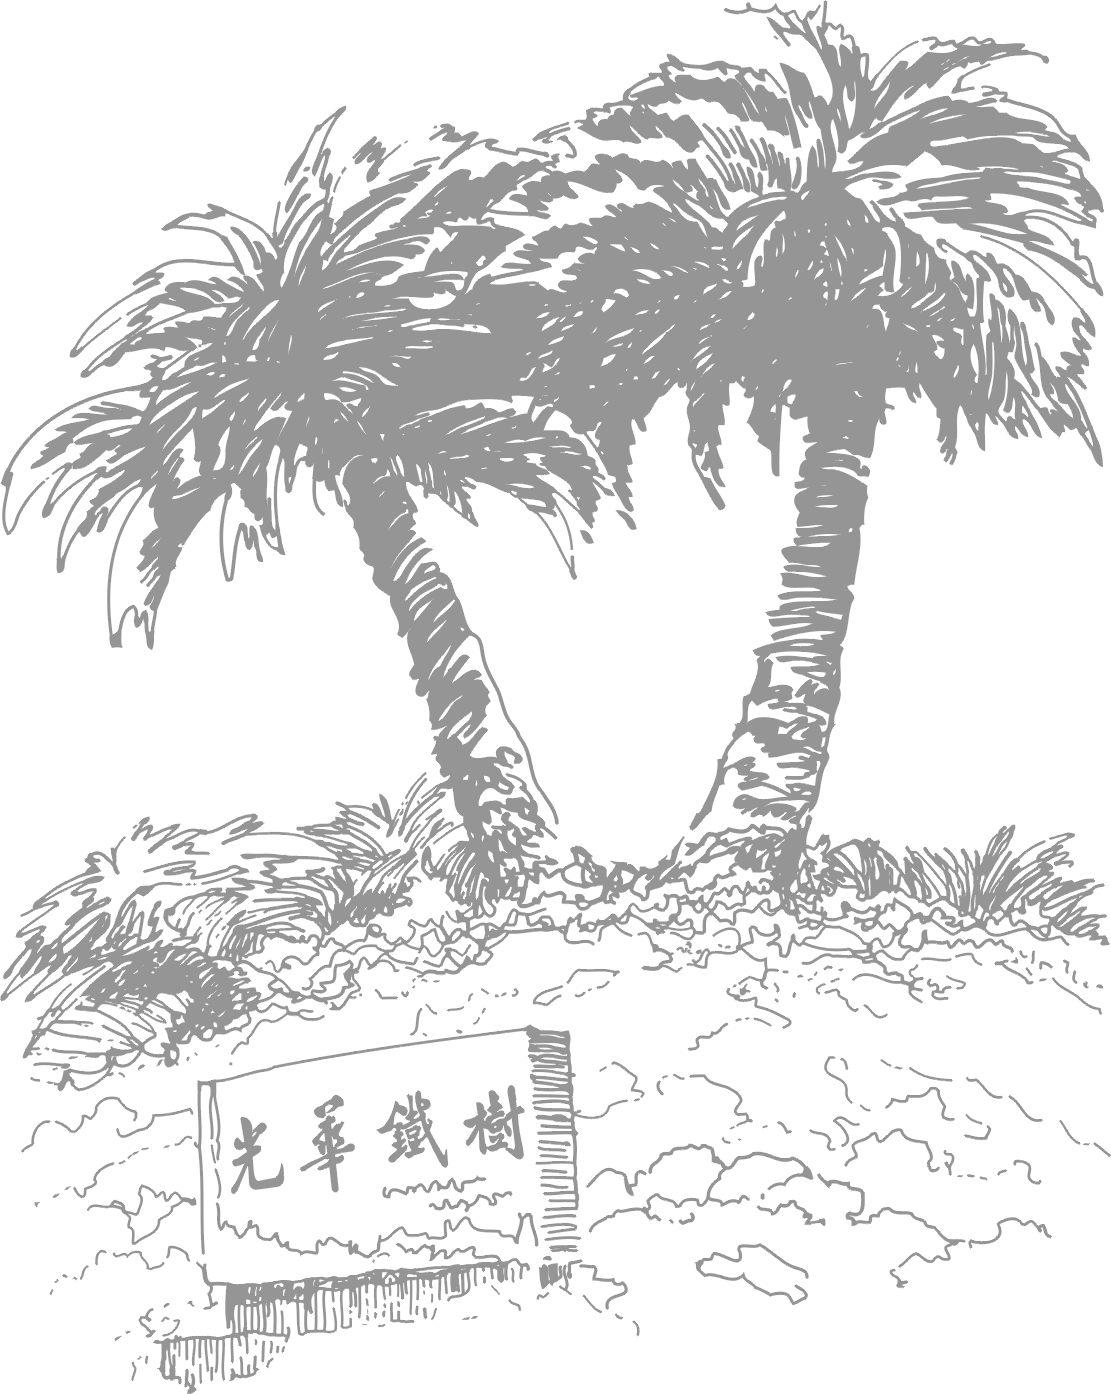
\includegraphics[width=11.5cm]{figures/swufe_cycad.png}
    };
    % 竖排校训“经世济民 孜孜以求”
    \node[anchor=center, xshift=1.0cm, yshift=1.8cm] at (current page.center) {
      \hwxingkai\fontsize{48pt}{56pt}\selectfont
      \begin{tabular}{c@{\hspace{1.8cm}}c}
        \parbox[t]{2em}{\linespread{1.1}\selectfont 孜\\孜\\以\\求} &
        \parbox[t]{2em}{\linespread{1.1}\selectfont 经\\世\\济\\民}
      \end{tabular}
    };
  \end{tikzpicture}%
  \null\clearpage
}

% ---------------------------------------------------------
% 16. 中英文摘要专属宏定义与格式规范
% ---------------------------------------------------------
\ExplSyntaxOn
% 覆盖 keywords 格式，中文以“；”分隔，末尾无标点
\cs_set_protected:Npn \__sjtu_keywords_format:n #1
  {
    \par\noindent
    \normalfont\songti\zihao{-4}\bfseries #1
  }

\tl_set:Nn \c__sjtu_name_item_sep_zh_tl { ； }
\tl_set:Nn \c__sjtu_name_item_sep_en_tl { ;~ }
\tl_set:Nn \c__sjtu_name_keywords_en_tl { Keywords }
\tl_set:Nn \c__sjtu_name_abstract_en_tl { ABSTRACT }
\ExplSyntaxOff

\makeatother
